\documentclass[border=15pt, multi, tikz]{article}
\usepackage{amssymb}
\usepackage[backend=bibtex,style=authoryear,natbib=true]{biblatex} % Use the bibtex backend with the authoryear citation style (which resembles APA)

\addbibresource{example.bib} % The filename of the bibliography

\usepackage[autostyle=true]{csquotes} % Required to generate language-dependent quotes in the bibliography
\usepackage{import}
\usepackage{tikz}
\usepackage{tikz-network}
\usetikzlibrary{calc,patterns,angles,quotes}
\usepackage{breqn}
\usepackage{bm}
\usepackage{graphicx}
\usepackage{subcaption}
\usepackage{multirow}
\usepackage{graphicx}
\usetikzlibrary{fit}
\usetikzlibrary {arrows.meta,graphs,shapes.misc}
\usetikzlibrary {positioning}
\subimport{./layers/}{init}
\newcommand{\bn}{\textbf{n}}
\newcommand{\tabhead}[1]{\textbf{#1}}

\def\ConvColor{rgb:yellow,5;red,2.5;white,5}
\def\ConvReluColor{rgb:yellow,5;red,5;white,5}
\def\PoolColor{rgb:red,1;black,0.3}
\def\DcnvColor{rgb:blue,5;green,2.5;white,5}
\def\SoftmaxColor{rgb:magenta,5;black,7}
\def\SumColor{rgb:blue,5;green,15}
\def\poolsep{1}


\begin{document}
	
\section{Guided normal inference using GCNN}

\subsection{Intrinsic image decomposition}
Intrinsic image model was introduced by \cite{intrinsic-image}. It interprets that an image $ I $ can be decomposed as the element-wise product between the reflectance $ R $ of the object and the shading $ S $ produced by the interaction between light and objects.
\[ I =R  \odot S\]
It interprets the observed image into reflectance image and the shading image. As shown in Figure \ref{fig:intrinsic-image}
%% insert a image for decompositions
\begin{figure}[th]
	\centering
	{\includegraphics[width=.18\textwidth]{./Figures/intrinsic_image.png}}
	{\includegraphics[width=.18\textwidth]{./Figures/intrinsic_image_reflectance.png}}
	{\includegraphics[width=.18\textwidth]{./Figures/intrinsic_image_shading.png}}
	{\includegraphics[width=.18\textwidth]{./Figures/intrinsic_image_light.png}}
	{\includegraphics[width=.18\textwidth]{./Figures/intrinsic_image_normal.png}}
	\caption{Intrinsic image analysis of the bus object. From left to right, original image, reflectance image, shading image, light image, normal image}
	\label{fig:intrinsic-image}
\end{figure}

The equation can be further decomposed based on different surface models. If assume the object surfaces are Lambertian surfaces, i.e. the surface which reflect light in all directions, the shading image can be decomposed as the product of the  radiance of  incoming light $ L_0 $, the cosine of the angle of incidence, which is the dot product of the surface normal $ N $ and the light source direction $ L $.
\[ I = \rho  \odot ( L_0 \textbf{L} \cdot  \textbf{N}) \]
note that the surface normal $ N $ and light direction $ L $ are unit vectors thus they have only two degrees of freedom. 

\begin{figure}[th]
	\centering
	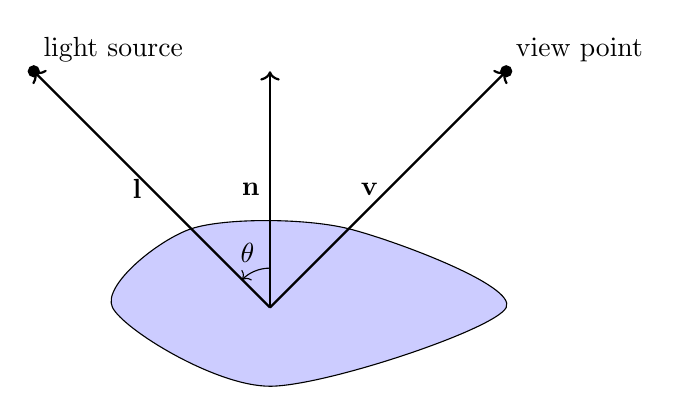
\begin{tikzpicture} 
		% reference lines
		\coordinate (light) at (-1,3);
		\coordinate (p) at (2,0);
		\coordinate (normal) at (2,3);
		\draw [fill=blue!20] plot [smooth cycle] coordinates {(0,0) (1,1) (3,1) (5,0) (2,-1)}; %% surface element
		\draw[thick, ->] (2,0) -- (2,3) node[midway, left] {$ \textbf{n} $}; %% normal
		\draw[thick, ->] (2,0) -- (-1,3) node[midway, left] {$ \textbf{l} $}  ; %% source direction
		\pic [draw, ->, "$\theta$", angle eccentricity=1.5] {angle = normal--p--light};
		\draw[thick, ->] (2,0) -- (5,3) node[midway, left] {$ \textbf{v} $}; %% view direction
		\filldraw[black] (-1,3) circle (2pt) node[anchor=south west]{light source}; %% light source
		\filldraw[black] (5,3) circle (2pt) node[anchor=south west]{view point}; %% view point		
	\end{tikzpicture}
	\caption{The surface normal, source light direction and the view point direction, where $ \theta $ denotes the angle between light direction and the normal.}
	\label{fig:lambertian-surface}
\end{figure}

The equation can be further rearranged as follows
\[ I = \textbf{g} \cdot \textbf{L} =(L_0\rho \odot \textbf{N}) \cdot  ( \textbf{L}) \]
The shape from shading method employed the equation mentioned above to predict the both surface albedo $ \rho $ and the normal $ \textbf{N} $ with knowning light source direction $ \textbf{L} $. More specifically, a set of $ k $ image for the same scene have been captured based on different light projections. Then, for each pixel $ (x,y) $ in the image, an equation system can be set up 

\[ 
\begin{pmatrix}
	L_1^T \\
	L_2^T \\
	\cdots \\
	L_k^T
\end{pmatrix} g(x,y) = 
\begin{pmatrix}
	I_1(x,y) \\
	I_2(x,y) \\
	\cdots \\
	I_3(x,y)
\end{pmatrix}
\]
for the simplicity, $ L_i^T $ for $ 1\le i \le k $ denotes the light direction at position $ (x,y) $ in the image $ k $ 
The equation can be solved based on least square methods. 
Since normal $ N(x,y) $ is unit vector, thus we have 

\[ \|g(x,y)\|_2 = \|L_0\rho(x,y)N(x,y)\|_2 = L_0\rho(x,y) \]

Then the normal can be obtained as follow

\[  N(x,y) = \frac{g(x,y)}{L_0\rho(x,y)}\]

In another word, the surface normal including the albedo can be obtained directly based on images and light directions. 


\subsection{Light Map}
The light map $ L $ can be derived from vertex map and the light source position. As shown in Figure \ref{fig:lambertian-surface}, the incoming light direction is a vector point from light source to the surface point, therefor it can be calculated as follows
\begin{equation}\label{light-direction}
	\begin{array}{ll}
		L(x,y)&= \frac{V(x,y)-(s_x,s_y)}{\|V(x,y)-(s_x,s_y)\|_2}\\ 
	\end{array}
\end{equation}
where $ (s_x,s_y) $ is the light source position and $ V $ is the vertices, both $  (s_x,s_y) $ and  $ V $ are with respect to the camera space. The light direction map $ L $ is normalized since only the direction of the light is considered. 
The light map is a matrix corresponding the light direction of whole image where each pixel corresponding with each other, thus it has the same size as the vertex map.


It is important to note that due to the exist noise in the vertex map, the getting light map is only semi-dense, as shown in Figure \ref{fig:light-input}. 

\begin{figure}[th]
	\centering
	{\includegraphics[width=.4\textwidth]{./Figures/intrinsic_image_vertex_input.png}}
	{\includegraphics[width=.4\textwidth]{./Figures/intrinsic_image_light_input.png}}
	\caption{The light map calculated from vertex map and the light source}
	\label{fig:light-input}
\end{figure}

In order to ease this issue, a light inpainting model has been trained based on the GCNN network with the identity architecture but the input and output, which takes the semi-dense light map as input and predict the fully dense light map as output. 

\begin{figure}[th]
	\centering
	%% https://tex.stackexchange.com/questions/12020/what-is-the-easiest-way-to-draw-a-3d-cube-with-tikz
	\begin{tikzpicture}
		%% -------------------------------------- parameters ------------------------------------------------
		\pgfmathsetmacro{\vdist}{0.4}
		
		\pgfmathsetmacro{\boxsizea}{2}	%% width 512
		\pgfmathsetmacro{\boxwidtha}{2}	%% width 3
		
		%% https://www.tug.org/pracjourn/2007-4/walden/color.pdf
		\definecolor{netcolor}{rgb}{0.5,0.7,0.7}
		
		%% 	d_in							3x512x512
		%%	dconv1: 	d_in-->x1 			32x512x512
		\pgfmathsetmacro{\disttimes}{1}	%% width 32
		\pgfmathsetmacro{\yshift}{1}	%% width 32
		\pgfmathsetmacro{\boxsize}{\boxsizea}	%% size 512
		\pgfmathsetmacro{\boxwidth}{\boxwidtha}	%% width 32
		\pgfmathsetmacro{\yschift}{-1}


		\node[inner sep=0pt] (input) at (\vdist*\disttimes-6,\yschift-0.8)
		{\includegraphics[width=.2\textwidth]{./Figures/intrinsic_image_light_input.png}};
		\node[text width=3.5cm] at (\vdist*\disttimes-6,\yschift-2.4) {Semi-dense Light Map};
		
		\node[inner sep=0pt] (output) at (\vdist*\disttimes+3,\yschift-0.8)
		{\includegraphics[width=.2\textwidth]{./Figures/intrinsic_image_light.png}};
		\node[text width=3.5cm] at (\vdist*\disttimes+3,\yschift-2.4) {Semi-dense Light Map};
		
		\draw [-stealth] (\vdist*\disttimes-4.5,\yschift-1) -- (\vdist*\disttimes-3.5,\yschift-1);
		\draw [-stealth] (\vdist*\disttimes,\yschift-1) -- (\vdist*\disttimes+1,\yschift-1);
		

		\pgfmathsetmacro{\disttimes}{-2}	%% width 32		
		\pgfmathsetmacro{\yschift}{-1}
		\draw[black, fill=netcolor] (\vdist*\disttimes,\yschift,0) -- ++(-\boxwidth,0,0) -- ++(0,-\boxsize,0) -- ++(\boxwidth,0,0) -- cycle;
		\draw[black, fill=netcolor] (\vdist*\disttimes,\yschift,0) -- ++(0,0,-\boxsize) -- ++(0,-\boxsize,0) -- ++(0,0,\boxsize) -- cycle;
		\draw[black, fill=netcolor] (\vdist*\disttimes,\yschift,0) -- ++(-\boxwidth,0,0) -- ++(0,0,-\boxsize) -- ++(\boxwidth,0,0) -- cycle;
		
		\node[text width=3.5cm] at (\vdist*\disttimes,\yschift-1) {Light Net};
\end{tikzpicture}
\caption{Light Net for light inpainting based on GCNN architecture.}
\label{fig:light-net-archi}
\end{figure}


\subsection{Light and image guided normal inference using GCNN}
Based on above implementations, we propose a Three branches Gated Convolutional Neural Network (TriGNet) to perform guided normal inference. The structure is shown in Figure \ref{fig:albedo-gated-archi}. As shown in the name, the network utilizes the GCNN architecture three times to accomplish the task. 

\begin{figure}[th]
	\centering 
	\begin{tikzpicture}
		\tikzstyle{connection}=[ultra thick,every node/.style={sloped,allow upside down},draw=\edgecolor,opacity=0.6]	
		
%%%%%%%%%%%%%%%%%%%%%%%%%%%%%%%%%%%%%%%%%%%%%%%%%%%%%%%%%%%%%%%%%%%%%%%%%%%%%%%%%%%%%%%%
%% Draw Layer Blocks
%%%%%%%%%%%%%%%%%%%%%%%%%%%%%%%%%%%%%%%%%%%%%%%%%%%%%%%%%%%%%%%%%%%%%%%%%%%%%%%%%%%%%%%%
% conv1_1,conv1_2,%pool1
\pic[shift={(0,0,0)}] at (0,0,0) {RightBandedBox={name=cr1,%
		xlabel={{"64","64"}},zlabel=I,fill=\ConvColor,bandfill=\ConvReluColor,%
		height=40,width={2,2},depth=40}};
\pic[shift={(\poolsep,0,0)}] at (cr1-east) {Box={name=p1,%
		fill=\PoolColor,opacity=0.5,height=30,width=1,depth=30}};
% conv2_1,conv2_2,pool2
\pic[shift={(1,0,0)}] at (p1-east) {RightBandedBox={name=cr2,%
		xlabel={{"64","64"}},zlabel=I/2,fill=\ConvColor,bandfill=\ConvReluColor,%
		height=30,width={3,3},depth=30}};
\pic[shift={(\poolsep,0,0)}] at (cr2-east) {Box={name=p2,%
		fill=\PoolColor,opacity=0.5,height=23,width=1,depth=23}};
% conv3_1,conv3_2,pool3
\pic[shift={(1,0,0)}] at (p2-east) {RightBandedBox={name=cr3,%
		xlabel={{"256","256","256"}},zlabel=I/4,fill=\ConvColor,bandfill=\ConvReluColor,%
		height=23,width={4,4,4},depth=23}};
\pic[shift={(\poolsep,0,0)}] at (cr3-east) {Box={name=p3,%
		fill=\PoolColor,opacity=0.5,height=14,width=1,depth=14}};
% conv4_1,conv4_2,conv4_3,pool4
\pic[shift={(1,0,0)}] at (p3-east) {RightBandedBox={name=cr4,%
		xlabel={{"512","512","512"}},zlabel=I/8,fill=\ConvColor,bandfill=\ConvReluColor,%
		height=14,width={7,7,7},depth=14}};
\pic[shift={(\poolsep,0,0)}] at (cr4-east) {Box={name=p4,%
		fill=\PoolColor,opacity=0.5,height=8,width=1,depth=8}};
% conv5_1,conv5_2,conv5_3,pool5
\pic[shift={(1,0,0)}] at (p4-east) {RightBandedBox={name=cr5,%
		xlabel={{"512","512","512"}},fill=\ConvColor,bandfill=\ConvReluColor,%
		height=8,width={7,7,7},depth=8}};
%% fc8 -> cr8 (score32)
\pic[shift={(0,0,0)}] at (cr5-east) {Box={name=score16,%
		xlabel={{"K","dummy"}},fill=\ConvColor,%
		height=8,width=2,depth=8,zlabel=I/16}};

%% Upsampling Deconv Layer
%% Dcnv16    
\pic[shift={(2.5,0,0)}] at (score16-east) {Box={name=d16,%
		xlabel={{"","dummy"}},fill=\DcnvColor,opacity=0.7,height=40,width=0.5,depth=40}};
%% Dcnv8    
\pic[shift={(.25,0,0)}] at (d16-east) {Box={name=d8,%
		xlabel={{"","dummy"}},fill=\DcnvColor,opacity=0.7,height=40,width=0.5,depth=40}};
%% Dcnv4    
\pic[shift={(.25,0,0)}] at (d8-east) {Box={name=d4,%
		xlabel={{"","dummy"}},fill=\DcnvColor,opacity=0.7,height=40,width=0.5,depth=40}};
%% Dcnv2    
\pic[shift={(.25,0,0)}] at (d4-east) {Box={name=d2,%
		xlabel={{"","dummy"}},fill=,opacity=0.01,height=40,width=0.5,depth=40}};

%% Dcnv envelope    
\pic[shift={(-0.2,0,0)}] at (d16-west) {Box={name=env,caption=concatenation of deconvolved feature maps,%
		xlabel={{"","dummy"}},fill=,opacity=0.2,height=42,width={8},depth=42}};
%%%%%%%%%%%%%%%%%%%%%%%%%%%%%%%%%%%%%%%%%%%%%%%%%%%%%%%%%%%%%%%%%%%%%%%%%%%%%%%%%%%%%%%%
\def\skipshift{6.5}
%%Joining with previous streams (fcn-16)
%% score16
\pic[shift={(0,0,3+\skipshift)}] at (cr5-anchor) {Box={name=score8,%
		xlabel={{"K","dummy"}},fill=\ConvColor,height=14,width=2,depth=14,zlabel=I/8}};
%%%%%%%%%%%%%%%%%%%%%%%%%%%%%%%%%%%%%%%%%%%%%%%%%%%%%%%%%%%%%%%%%%%%%%%%%%%%%%%%%%%%%%%%
%%Joining with previous streams (fcn-8)
%% score8
\pic[shift={(0,0,8+\skipshift)}] at (cr4-east) {Box={name=score4,%
		xlabel={{"K","dummy"}},fill=\ConvColor,height=23,width=2,depth=23,zlabel=I/4}};
%%%%%%%%%%%%%%%%%%%%%%%%%%%%%%%%%%%%%%%%%%%%%%%%%%%%%%%%%%%%%%%%%%%%%%%%%%%%%%%%%%%%%%%%
%%Joining with previous streams (fcn-4)
%% score4
\pic[shift={(1,0,13+\skipshift)}] at (cr3-east) {Box={name=score2,%
		xlabel={{"K","dummy"}},fill=\ConvColor,height=30,width=2,depth=30,zlabel=I/2}}; 
%%%%%%%%%%%%%%%%%%%%%%%%%%%%%%%%%%%%%%%%%%%%%%%%%%%%%%%%%%%%%%%%%%%%%%%%%%%%%%%%%%%%%%%%
%%Joining with previous streams (fcn-2)
%% score2
\pic[shift={(0.3,0,22+\skipshift)}] at (p2-east) {Box={name=score,%
		xlabel={{"K","dummy"}},fill=\ConvColor,height=40,width=2,depth=40,zlabel=I}};
%%%%%%%%%%%%%%%%%%%%%%%%%%%%%%%%%%%%%%%%%%%%%%%%%%%%%%%%%%%%%%%%%%%%%%%%%%%%%%%%%%%%%%%%
% Final convolution

\pic[shift={(3,0,0)}] at (d2-east) {Box={name=output,%
		xlabel={{"K","dummy"}},fill=\ConvColor,height=40,width=2,depth=40,zlabel=I}};
%%%%%%%%%%%%%%%%%%%%%%%%%%%%%%%%%%%%%%%%%%%%%%%%%%%%%%%%%%%%%%%%%%%%%%%%%%%%%%%%%%%%%%%%%
%%% Draw connections
%%%%%%%%%%%%%%%%%%%%%%%%%%%%%%%%%%%%%%%%%%%%%%%%%%%%%%%%%%%%%%%%%%%%%%%%%%%%%%%%%%%%%%%%%
\draw [connection]  (cr1-east)    -- node {\midarrow} (p1-west);
\draw [connection]  (p1-east)    -- node {\midarrow} (cr2-west);
\draw [connection]  (cr2-east)    -- node {\midarrow} (p2-west);
\draw [connection]  (p2-east)    -- node {\midarrow} (cr3-west);
\draw [connection]  (cr3-east)    -- node {\midarrow} (p3-west);
\draw [connection]  (p3-east)    -- node {\midarrow} (cr4-west);
\draw [connection]  (cr4-east)    -- node {\midarrow} (p4-west);
\draw [connection]  (p4-east)    -- node {\midarrow} (cr5-west);
\draw [connection]  (score16-east)    -- node {\midarrow} (d16-west);
%
\path (cr4-east) -- (p4-west) coordinate[pos=0.4] (after4) ;
\draw (d16-near)++(0,0,-1+\skipshift) coordinate (d16h);
\draw [connection]  (after4)    -- node {\midarrow} ++(0,0,3+\skipshift) -- node {\midarrow} (score8-west);
\draw [connection]  (score8-east) -- node{\midarrow} (d16h) -- node{\midarrow}(d16-near);
%
\path (cr3-east) -- (p3-west) coordinate[pos=0.4] (after3) ;
\draw (d8-near)++(0,0,4+\skipshift) coordinate (d8h);
\draw [connection]  (after3)    -- node {\midarrow} ++(0,0,8+\skipshift) -- node {\midarrow} (score4-west);
\draw [connection]  (score4-east) -- node{\midarrow} (d8h) -- node{\midarrow}(d8-near);
%
\path (cr2-east) -- (p2-west) coordinate[pos=0.4] (after2) ;
\draw (d4-near)++(0,0,9+\skipshift) coordinate (d4h);
\draw [connection]  (after2)    -- node {\midarrow} ++(0,0,13+\skipshift) -- node {\midarrow} (score2-west);
\draw [connection]  (score2-east) -- node{\midarrow} (d4h) -- node{\midarrow}(d4-near);
%
\path (cr1-east) -- (p1-west) coordinate[pos=0.4] (after1) ;
\draw (d2-near)++(0,0,18+\skipshift) coordinate (d2h);
\draw [connection]  (after1)    -- node {\midarrow} ++(0,0,22+\skipshift) -- node {\midarrow} (score-west);
\draw [connection]  (score-east) -- node{\midarrow} (d2h) -- node{\midarrow}(d2-near);

\draw [connection]  (d2-east)    -- node {\midarrow} (output-west);
%%%%%%%%%%%%%%%%%%%%%%%%%%%%%%%%%%%%%%%%%%%%%%%%%%%%%%%%%%%%%%%%%%%%%%%%%%%%%%%%%%%%%%%%
	\end{tikzpicture}
	\caption{TriGNet Architecture}
	\label{fig:trig-net-archi}
\end{figure}



\end{document}
